\documentclass[11pt, oneside]{article} 
\usepackage{geometry}
\geometry{letterpaper} 
\usepackage{graphicx}
	
\usepackage{amssymb}
\usepackage{amsmath}
\usepackage{parskip}
\usepackage{color}
\usepackage{hyperref}

\graphicspath{{/Users/telliott_admin/Tex/png/}}
% \begin{center} 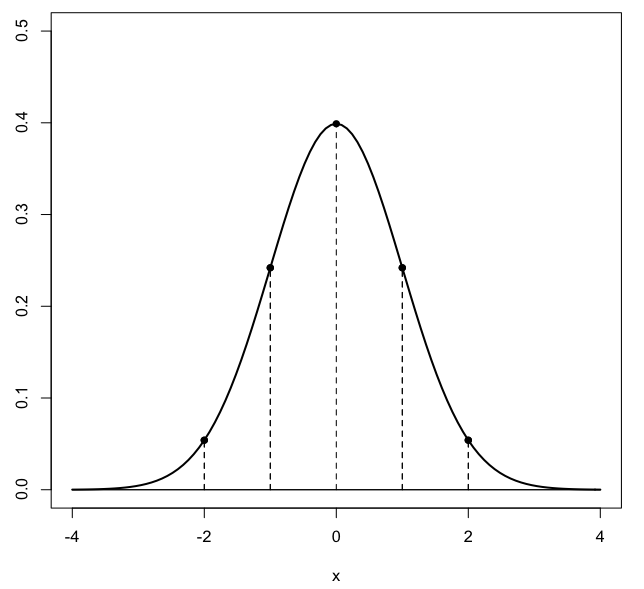
\includegraphics [scale=0.4] {gauss3.png} \end{center}

\title{The Divergence}
\date{}

\begin{document}
\maketitle
\Large

In the two previous chapters we worked out Green's Theorem, which relates line integrals in the plane to double integrals over the included region.  Each version of Green's Theorem has a short-hand vector expression, together with another differential version in which the meaning is more explicit.  

The theorem for work is
\[ \oint \mathbf{F} \cdot d \mathbf{r} = \iint_R \nabla \times \mathbf{F} \ dA \]
alternatively
\[ \int_C M \ dx + N \ dy = \iint_R N_x - M_y \ dx \ dy \]

The work done along a closed path $C$ around a region $R$ is equal to the double integral over $R$ of the curl of $\mathbf{F}$.  If $\mathbf{F}$ is a whirlpool then work will be done, if the force is conservative there is no net circulation and the total work will be zero.

The theorem for flux is
\[ \oint \mathbf{F} \cdot  \mathbf{\hat{n}} \ ds  = \iint_R \nabla \cdot \mathbf{F} \ dA \]
Recall that $d\mathbf{r} = \mathbf{\hat{T}} \ ds$ and $\mathbf{\hat{T}}$ is orthogonal to $\mathbf{\hat{n}}$ so
\[ \int_C M \ dy - N \ dx = \iint_R M_x + N_y \ dx \ dy \]

I think that using $\nabla \cdot \mathbf{F}$ and $\nabla \times \mathbf{F}$ is not technically correct in $\mathbb{R}^2$, (one should rather say "div F" and "curl F"), since $\nabla$ really lives in three dimensions.  As discussed previously, for the curl what we are effectively doing is taking a cross product (with the field zero in the $z$ direction), then using the dot product with $\mathbf{\hat{k}}$.  

For the divergence, it may be better to move now to three dimensions for discussion of the analogous theorem, sometimes ascribed to Gauss, although there are other claimants.

\subsection*{Divergence}

In $\mathbb{R}^3$ we write:
\[ \iint_S \mathbf{F} \cdot \mathbf{\hat{n}} \ dS  = \iiint_V \ \nabla \cdot \mathbf{F} \ dV \]
\[ =  \iiint_V \ (P_x + Q_y + R_z )\ dV \]

As a simple example, consider the unit sphere and a radial field $\mathbf{F} = \langle x,y,z \rangle$.  In this case, we can do the surface integral because of the radial symmetry.  

Clearly the force and the surface normal are parallel everywhere, because, for any $x,y,z$ on the surface of the sphere, the vector to that point is $\langle x,y,z \rangle$ and so is the force at that point.

Therefore, everywhere on the surface, $\mathbf{F}$ is in the same direction as the normal, so
\[ \mathbf{F} \cdot \mathbf{\hat{n}} = F \]

We have $F$ times the surface area of the unit sphere.

Everywhere on the unit sphere $F = 1$.  We can see this easily for three points $(1,0,0)$, $(0,1,0)$, and $(0,0,1)$.  

In general we have $z^2 = 1 - x^2 - y^2$ so
\[ F = | \mathbf{F} | = \sqrt{\mathbf{F} \cdot \mathbf{F}} \]
\[ =   \sqrt{x^2 + y^2 + + z^2} \]
\[ =   \sqrt{ x^2 + y^2 + 1 - x^2 - y^2} = 1 \]
We multiply by the surface area of the unit sphere and obtain $4 \pi$.

To check this using the right-hand side of the divergence equation, notice that 
\[ \nabla \cdot \mathbf{F} = P_x + Q_y + R_z = 3 \]
Using the theorem, the result (the flux out of the sphere) is simply $3$ times the volume of the unit sphere, or finally, $4 \pi$.  The result is the same.

\subsection*{Other coordinates}

The divergence was given as
\[ \iiint_V \ \nabla \cdot \mathbf{F} \ dV \]

The "del" operator is
\[ \nabla = \ < \frac{\partial}{\partial x},\frac{\partial}{\partial y},\frac{\partial}{\partial z} > \]
The divergence of $\mathbf{F}$ is
\[ \nabla \cdot \mathbf{F} \]
if $\mathbf{F} = \ <P,Q,R>$
\[ \nabla \cdot \mathbf{F} = P_x + Q_y + R_z \]
The divergence of a vector field is a scalar quantity.

Although the expression above is often given as the \emph{definition} of divergence, Schey makes a big deal out of saying that he prefers another definition

\[ div \ \mathbf{F} = \lim_{\Delta V \rightarrow 0} \frac{1}{\Delta V} \iint_S \ \mathbf{F} \cdot \hat{\mathbf{n}} \ dS \]

This can be used to derive expressions for the divergence in cylindrical and spherical coordinates, where it has a more complicated form.  In cylindrical coordinates: 

\[ div \ \mathbf{\mathbf{F}} = \frac{1}{r} \frac{\partial}{\partial r} (rF_r) +  \frac{1}{r} \frac{\partial}{\partial \theta} (F_{\theta}) + \frac{\partial}{\partial z} (F_z) \]

(Here $F_{z}$ is not a partial derivative but just the component of $\mathbf{F}$ in the z-direction, and so on).

Similarly, in spherical coordinates the divergence is

\[ div \  \mathbf{\mathbf{F}} = \frac{1}{r^2} \frac{\partial}{\partial r} (r^2F_r) +  \frac{1}{r \ \sin \phi} \frac{\partial}{\partial \phi} (\sin \phi F_{\phi}) + \frac{1}{r \ \sin \phi} \frac{\partial}{\partial \theta} (F_{\theta}) \]

There are other people who say this makes much more sense, but exploring the consequences seems beyond what I want to do here.

\url{http://math.oregonstate.edu/BridgeBook/book/guide/thm}

\subsection*{cylindrical example}

Let's look at a few examples to explore divergence in cylindrical coordinates.  Suppose we have a cylinder oriented along the $z$-axis with its length equal to $1$ and its radius $r=2$.  

Further, we have a field with some divergence, like $\mathbf{F} = \langle x,y,0 \rangle$.

This field is written in $x,y,z$ coordinates, when we switch to cylindrical coordinates
\[ x = r \cos \theta \]
\[ y = r \sin \theta \]

We want to check the divergence theorem by computing both sides of
\[ \iint_S \mathbf{F} \cdot \mathbf{n} \ dS  = \iiint_V \ \nabla \cdot \mathbf{F} \ dV \]

The double integral is an integral over a closed surface, in this case, the cylinder with top and bottom included. 

When we rewrite $\mathbf{F}$ in cylindrical coordinates, we will have 
\[ \mathbf{F} = \langle r, \theta, z \rangle \]
The given field is independent of $\theta$ and $z$ and and since
\[ r = \sqrt{x^2 + y^2} \]
\[ \mathbf{F} = \langle r, 0, 0 \rangle \]

Using the definition of divergence from above, we have
\[ div \ \mathbf{\mathbf{F}} = \frac{1}{r} \frac{\partial}{\partial r} (rF_r) +  \frac{1}{r} \frac{\partial}{\partial \theta} (F_{\theta}) + \frac{\partial}{\partial z} (F_z) \]
since $\mathbf{F}$ has no $z$ or $\theta$ component and the $r$ component is $F_r =r$ (this is \emph{not} a derivative), we have  
\[ div \ \mathbf{\mathbf{F}} = \frac{1}{r} \frac{\partial}{\partial r} (r^2) = 2 \]

So the triple integral uses the cylindrical volume element and is just
\[ \int_0^{2 \pi} \ \int_0^{1} \ \int_0^2 \ 2 \ r \ dr \ dz \ d \theta  \]
\[ = \int_0^{2 \pi} \ \int_0^{1} \ [ \ r^2 \ \bigg |_0^2 \ ] \ dz \ d \theta = 8 \pi \]

Notice that the value of the volume integral scales linearly with $z$ and like $r^2$.

Now for the surface integral.  In standard form, on the sides, the cylinder has 
\[ \hat{\mathbf{n}} \ dS = \mathbf{r} \ d \theta \ dz = \langle x, y, 0 \rangle \ d \theta \ dz \]
\[  \iint_S \mathbf{F} \cdot \mathbf{n} \ dS  = \iint_S \langle x, y, 0 \rangle \cdot \langle x, y, 0 \rangle \ d \theta \ dz \]
\[  \iint_S x^2 + y^2  \ d \theta \ dz \]
\[  \int_0^1 \ \int_0^{2 \pi} \ r^2  \ d \theta \ dz = 2 \pi r^2 = 8 \pi \]

Don't forget the top and bottom of the cylinder.  However, since the force is radial, the flux $\mathbf{F} \cdot \hat{\mathbf{n}} = 0$ everywhere on these two surfaces, so the total is still just $8 \pi$.

\subsection*{spherical example}
Verify the divergence theorem for a \emph{hemisphere} of radius $a$ with $\mathbf{F} = \langle x,y,z \rangle$.

First, restate the theorem
\[ \iint_S \ \mathbf{F} \cdot \hat{\mathbf{n}} \ dS = \iiint_D \ \nabla \cdot \mathbf{F} \]

In spherical coordinates, the surface area element is

\begin{center} 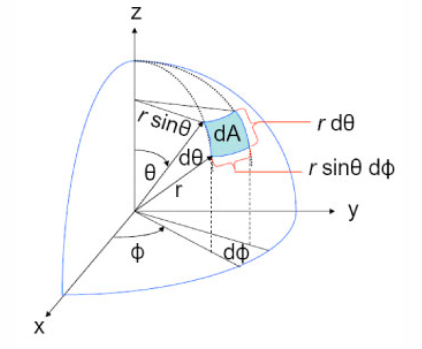
\includegraphics [scale=0.5] {sphere_ndS.png} \end{center} a "box" with sides
$r \ d \theta$ and $r \sin \phi \ d \phi$.  Here $r$ is given as $a$ so

\[ \hat{\mathbf{n}} \ dS = a^2  \ \sin \phi \ d \phi \ d \theta \]

The field was given in $x,y,z$-coordinates, $\mathbf{F} = \langle x,y,z \rangle$.  This is just $\mathbf{r}$.  Since $\mathbf{F}$ is orthogonal to the surface at every point the contribution of $\mathbf{F}$ to the dot product is $|\mathbf{F}| = a$, so we have
\[ \mathbf{F} \cdot \hat{\mathbf{n}} \ dS = a \cdot a^2  \ \sin \phi \ d \phi \ d \theta \]

and
\[ = \iint_S a^3  \ \sin \phi \ d \phi \ d \theta \]
This is a hemisphere so the bounds on $\phi$ are half the usual
\[ = a^3 \int  \ [ \ - \cos \phi \ \bigg |_0^{\pi/2}  \ ] \ d \theta \]
\[ = a^3  \int \ d \theta  = 2 \pi a^3 \]

Don't forget the bottom surface.  In this problem, there is a component of the field in the $z$ direction

\[ \mathbf{F} \cdot \hat{\mathbf{n}} \ dS =  \langle x,y,z \rangle \cdot  \langle 0,0,-1 \rangle \ dx \ dy = -z \ dx \ dy\]
however, the value of the field on the $xy$-plane is $z=0$ so there is no flux.

For the divergence,

\[ \nabla \cdot \mathbf{F} = 1 + 1 + 1 = 3 \]
which is pretty easy!.  Now, integrate
\[ \iiint_D \ 3 \ dV \]
Well, the volume is $\frac{2}{3} \pi a^3$ so we obtain $2 \pi a^3$, which matches.

\subsection*{OSU example}

A problem from OSU asks us to verify the divergence theorem for 
\[ \mathbf{F} = \ \langle y,x,z \rangle \]

where the region is
\[ 0 \le z \le 16 -x^2 -y^2 \]

The graph of $z=16 -x^2 -y^2$ is a paraboloid which opens downward and has its vertex at $z=16$.  When $z=0$ we have a circle of radius $r=4$.

Recall that 
\[ \hat{\mathbf{n}} \ dS = \langle -f_x,-f_y,1 \rangle  \ dA \]
 so for this paraboloid surface we have
 \[ z = f(x,y) = 16 - x^2 - y^2 \]
\[ \hat{\mathbf{n}} \ dS = \ \langle 2x,2y,1 \rangle  \ dA \]
This corresponds to $\hat{\mathbf{n}}$ pointing out of the surface.
Then
\[ \iint_S \mathbf{F} \cdot \hat{\mathbf{n}} \ dS  = \iint_R 4xy + z \ dA \]
\[ =  \int_{-4}^{4} \int_{-\sqrt{16-y^2}}^{\sqrt{16-y^2}} \ 4xy + 16 - x^2 - y^2 \ dx \ dy \]

$xy$-coordinates are not a good way to do this problem.  Convert to polar coordinates
\[ x = r \cos \theta \]
\[ y = r \sin \theta \]
\[ dA = r \ dr \ d\theta \]
\[  \iint_R (4r^2 \sin \theta \cos \theta + 16 - r^2) \ r \ dr \ d\theta \]
The region of integration is the disk of radius $r=4$
\[ \int_0^{2\pi} \ \int_0^4 \ (4 r^2 \sin \theta \cos \theta + 16 - r^2) \ r \ dr \ d \theta \]
The inner integral is
\[ \int_0^4 \ 4 r^3 \sin \theta \cos \theta + 16r - r^3 \ dr \]
\[ r^4  \sin \theta \cos \theta + 8r^2 - \frac{1}{4}r^4 \ \bigg |_0^4 \]
\[ = 256   \sin \theta \cos \theta + 128 - 64 \]
\[ = 256   \sin \theta \cos \theta + 64 \]
The outer integral is
\[ \int_0^{2\pi} 64 +  256  \sin \theta \cos \theta \ d \theta \]
\[ = 128 \pi + 256 \sin^2 \theta \bigg |_0^{2\pi} \]
\[ = 128 \pi  \]
There is another part of our solid.  That is the disk in the $xy$-plane.  For this disk, the unit normal (pointing out) is just $\langle 0,0,-1 \rangle$.
\[ \iint_S \mathbf{F} \cdot \hat{\mathbf{n}} \ dS  = -\iint_R z \ dA \]
but remember that we're on the $xy$-plane so $z=0$ and the whole integral is $0$.

We're not done yet!  We still have to compute
\[ \iiint_R \ \nabla \cdot \mathbf{F} \]
\[ = \iiint_R P_x + Q_y + R_z \ dV \]
since $\mathbf{F} = \ \langle y,x,z \rangle$ this is just equal to $3$.  So we need 
\[ 3 \iiint_R  \ dV \]
If we convert to cylindrical coordinates, we will integrate over the disk of radius $r=4$.  What is the upper bound on $z$?
\[ z = 16 - x^2 - y^2 = 16 - r^2 \]
So we have
\[ \int_0^{2\pi} \ \int_0^4 \ \int_0^{16 - r^2} \ dz \ r \ dr \ d \theta \]

The inner integral is just $16 - r^2$.  The middle integral is
\[ \int_0^4 16r - r^3 \ dr \]
\[ = 8r^2 - \frac{1}{4}r^4 \ \bigg |_0^4 \]
\[ = 128 - 64 = 64 \]
Finally, we pick up $2 \pi$ from the outer integral for a final result of $128 \pi$, which matches what we had above.

Or, we could have just said that the solid is a hemisphere of radius $4$ so the volume is a standard formula.  Again, we need 
\[ 3 \iiint_R  \ dV \]
so
\[ 3 V = 3 \ \frac{1}{2} \ \frac{4}{3} \pi 4^3 \]
$16^2 = 256$ and one-half of that is $128$, times $\pi$.

Conceptually, going from 2 to 3 dimensions doesn't seem like a big deal.  But the problems are considerably more challenging.

\end{document}